\begin{abcliste}
\abc With $e U = \frac{p^2}{2 m_e}$ and $\lambda = h/p$:
\begin{align}
 \lambda &= \laF \\
   &= \frac{\nch}{\sqrt{2\times\ncme\times\nce\times\UA}} \\
   &= \la \approx \result{\laP{-12}{3}}
\end{align}

\abc With $\lambda = \frac{h}{\sqrt{2 m_e e U}}$,
\begin{align}
 r &= \frac{L\,\lambda}{d} = \frac{L\,h}{d\,\sqrt{2 m_e e}}\cdot\frac{1}{\sqrt{U}} = k\cdot\frac{1}{\sqrt{U}}
\end{align}
so $r$ is proportional to $1/\sqrt{U}$: a line through the origin with the slope $k = \frac{L\,h}{d\,\sqrt{2 m_e e}}$.

\begin{center}
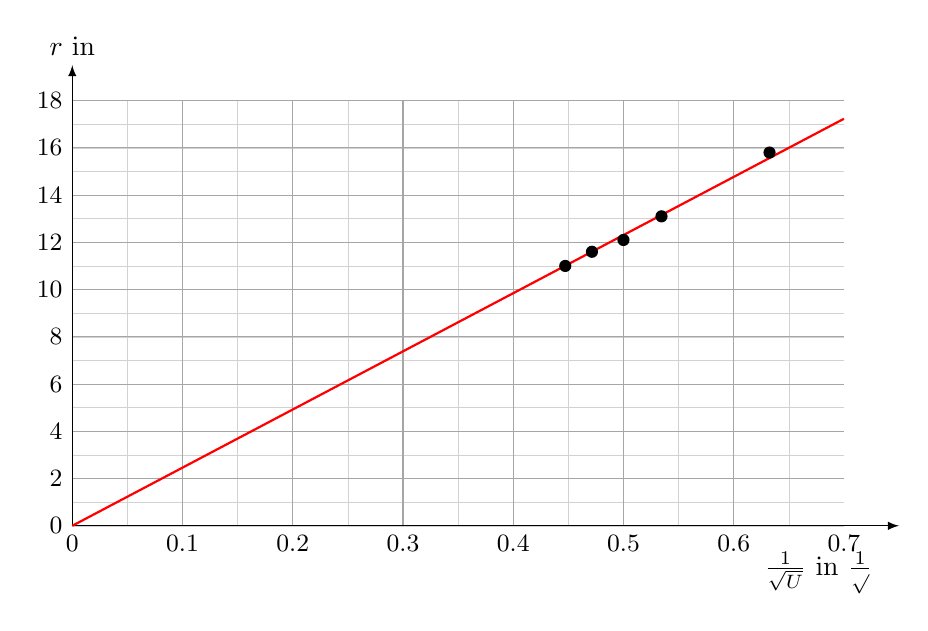
\begin{tikzpicture}[x=14cm, y=0.3cm, >=latex]
 \draw[gray!35, very thin] (0,0) grid[xstep=0.05, ystep=1] (0.7,18);
 \draw[gray!70] (0,0) grid[xstep=0.1, ystep=2] (0.7,18);
 \draw[->] (0,0) -- (0.75,0) node[below left=6pt] {$\frac{1}{\sqrt{U}}$ in $\frac{1}{\sqrt{\si{\kilo\volt}}}$};
 \draw[->] (0,0) -- (0,19.5) node[above] {$r$ in \si{\milli\meter}};
 \foreach \x in {0,0.1,0.2,0.3,0.4,0.5,0.6,0.7} \node[below] at (\x,0) {\small \x};
 \foreach \y in {0,2,...,18} \node[left] at (0,\y) {\small \y};
 \draw[red, thick] (0,0) -- (0.7,17.23);
 \fill (0.6325,15.8) circle (2.2pt);
 \fill (0.5345,13.1) circle (2.2pt);
 \fill (0.5000,12.1) circle (2.2pt);
 \fill (0.4714,11.6) circle (2.2pt);
 \fill (0.4472,11.0) circle (2.2pt);
\end{tikzpicture}
\end{center}

The line through the origin that fits the points best has the slope (read off the graph, or by least squares)
\begin{align}
 k &\approx \kmmP{0}{3}\,\si{\milli\meter}\sqrt{\si{\kilo\volt}} = \slP{0}{3}\,\si{\meter}\sqrt{\si{\volt}}
\end{align}
Solved for $d$:
\begin{align}
 d &= \dgF \\
   &= \frac{\Ls\times\nch}{\slP{0}{3}\,\si{\meter}\sqrt{\si{\volt}}\times\sqrt{2\times\ncme\times\nce}} \\
   &= \dg \approx \result{\dgP{-9}{2}}
\end{align}
That is the spacing of the planes in graphite, \SI{0.213}{\nano\meter}.

\abc $r \propto \lambda \propto 1/\sqrt{U}$: four times the voltage gives \result{\text{half the radius}}. That the rings shrink when the electrons get faster showed that they come from the waves of the electrons, not from X-rays made in the tube.
\end{abcliste}
